\newcommand{\MExp}{{\small \textsc{MExp}}}
\section{Background}
Here, we review the technical problem we are trying to solve as well as the details of \citet{schirmer2022modeling}'s
continuous recurrent unit (CRU). 
This lays a conceptual foundation for our later innovations that incorporate data-dependent missingness mechanisms in Sec.~\ref{sec:CRU_gen_model}.


\paragraph{Problem: Irregular time series with missingness.}
We consider building a model for many multivariate sequences.
%For each sequence, we first define $t_0$ as a special reference start time for each sequence (e.g. the moment of admission to the hospital).
For each sequence, we have observations at a set $\Gamma$ of $L$ distinct irregularly-spaced observation times: $\Gamma=\{ t_1, ..., t_L\}$, which we assume are sorted in ascending order and are all greater than a reference start time $t_0$.

We also have a sequence $\mathbf{x}$ of observed feature vectors, one for each observed time: $\mathbf{x} = \{x_t : t \in \Gamma \}$. 
Each feature vector $x_t \in \mathbb{R}^D$ represents measurements of a fixed set of $D$ variables (sometimes called channels). There may be arbitrary missingness in each $x_t$. 
Let $s_t \in \{0, 1\}^D$ be a binary indicator vector of size $D$ indicating whether a variable is ``seen'' (observed) or not (missing). That is, $s_{td} = 1$ if $x_{td}$ is observed and 0 otherwise.

\subsection{Continuous Recurrent Unit (CRU)}
\label{sec:CRU}

A core building block of our approach is the continuous-time recurrent unit (CRU) by \citet{schirmer2022modeling}. The purpose of the CRU is to provide a  mapping from a \emph{non-missing} irregular time series of length $L$ to a output sequence of representation vectors of the same length $L$. We write the CRU as
\begin{align}
    [h_{t_1} \ldots h_{t_L}], [\tau_{t_1} \ldots \tau_{t_L}] \gets \textsc{CRU}(x_{t_1} \ldots x_{t_L}, \Gamma).
    \label{eq:CRU_as_RNN}
\end{align}
At each observation time $t_\ell$, the CRU produces two $D$-dimensional vectors $h_{t_{\ell}}, \tau_{t_{\ell}}$. That is, $|h_t|{=}|\tau_t|{=}|x_t|{=}D$ for all $t \in \Gamma$. Vector $h_{t_\ell}$ is can be thought of as a decoded representation for data $x_{t_\ell}$.
Vector $\tau_{t_L}$ is meant to encode uncertainty about each data dimension.
%the representation vector and $\tau_t$ represents the uncertainty in the representations at time $t$.

We stress that the CRU as presented by \citet{schirmer2022modeling} assumes that each $x_t$ is fully observed, without any missingness. While they offer a zero-filling heuristic to accommodate missingness, our later experiments show this is inadequate for downstream predictions when data is missing-not-at-random. Instead, our methods in Sec.~\ref{sec:CRU_gen_model} provide an explicit mechanism to handle the data-dependent missingness scenarios.

\paragraph{CRU overview.}
The CRU produces representations via continuous-discrete Kalman-filter forward inference \citep{jazwinski2007stochastic} for a latent variable time-series model.
Internally, the CRU assumes two time-varying continuous random variables: a $M$-dimensional latent vector $z_t$, and a $C$-dimensional encoded feature vector $y_t$. Latent $z_t$ has a \emph{prior} distribution specified by a stochastic differential equation (SDE) model for $z_t$ as a function of $t$.
When this SDE assumes a Gaussian noise process, this ultimately yields a Gaussian prior with time-varying parameters.
%to a linear operation on the noise process
%The solution to the prior SDE in Eq.~\eqref{eq:LTI_SDE_soln} is a Gaussian distribution due to a linear operation on the noise process (which is itself Gaussian).  
We then define a Gaussian \emph{likelihood} that produces encoded features $y_t$ given latent $z_t$. Due to conjugacy between the solution to the prior SDE and the likelihood, \citet{jazwinski2007stochastic} shows that the posterior over $z_t$ given previously observations, $p( z_t | \{y_u : u < t, u \in \Gamma \})$, remains Gaussian with closed-form mean and covariance.

The CRU proceeds by mapping observed time series $x$ to encoded features $y$ and then employing forward Kalman-filter recursions to update the time-varying mean and covariances that summarize the posterior on latent $z$.
Later, a decoder neural network maps the posterior mean and uncertainty from the latent space to the $D$-dimensional data space, producing the sequence of $h$ and $\tau$ values in Eq.~\eqref{eq:CRU_as_RNN}.

We emphasize that although there is an underlying probabilistic model for $z$ and $y$, the actual CRU computations are all \emph{deterministic}, like any other recurrent neural net. Given an input sequence of data values $x$, the CRU will always produce the same latent means, latent covariances, and decoded data representations $h, \tau$.
Our later model thus treats the CRU as a flexible non-linear transformation function, like any other recurrent neural net.

\paragraph{CRU prior on $z$.}
The CRU model assumes a continuous latent vector $z\in \mathbb{R}^M$, which as a function of time $z(t)$ is governed by a linear time invariant (LTI) SDE
\begin{align}
    dz = Azdt + Gd\beta, ~~ p(z_{t_0})=\mathcal{N}(m_0, P_0),
    \label{eq:LTI_SDE}
\end{align}
where $A\in\mathbb{R}^{M\times M}$ is the time-invariant transition matrix, $G\in\mathbb{R}^{M\times B}$ is the diffusion coefficient and $\beta \in \mathbb{R}^B$ is a Brownian motion process (aka Wiener process) with zero mean and diffusion matrix $Q\in \mathbb{R}^{B\times B}$. The initial density condition (at time $t_0$) for the LTI-SDE is Gaussian, with $m_0$ and $P_0$ as the mean and covariance.

Following~\citet{sarkka2019applied}, the solution to Eq.~\eqref{eq:LTI_SDE} has the form
\begin{align}
    \label{eq:LTI_SDE_soln}
    z(t) &= \MExp(A(t-t_0))~z(t_0) + \int_{t_0}^t \MExp(A(t-\gamma))~G ~d\beta(\gamma) \notag
\end{align}
Here $\MExp$ refers to the matrix exponential, which maps a square matrix to another square matrix of the same size (details in the appendix). 
% \todo{See Supp. for details}.

\newcommand{\RRR}{R}

\paragraph{CRU likelihood of $y$ given $z$.}
The CRU model assumes that time-varying vector $y \in \mathbb{R}^C$ is generated by a Gaussian whose mean is a linear function of $z$
\begin{align*}
    y_t \mid z_t \sim \mathcal{N}(\RRR z_t, \sigma_t^2 I_C),
\end{align*}
where matrix $\RRR \in \mathbb{R}^{C \times M}$ and scalar $\sigma_t > 0$ are learnable parameters.

\paragraph{Posterior of $z$ given $y$.}
First, we can provide a formula for $p(z_t|y_{<t})$, our belief about $z_t$ using only previous observations of $y$ values:
\begin{align}
        p(z_t|y_{< t} )=\mathcal{N}(\mu^{-}_{t}, \Sigma^{-}_{t})
\end{align}
where $\mu_t^-$ and $\Sigma_t^{-}$ at time $t$ have analytical solutions \citep{sarkka2019applied} that depend 
also on the value $t'$ indicating the most recent previous observation time before $t$ in $\Gamma$: 
\begin{align}
    \label{eq:CRU_predict}
\mu_t^- &=
\begin{cases}
    \MExp(A(t-t'))m_0 & \text{if } t'=t_0, \\
    \MExp(A(t-t'))\mu_{t'}^+ & \text{if }t'>t_0    
\end{cases}
\\ \notag
\Sigma_t^{-} %= &\mathbb{E}[(z(t)-\mu_t^-)(z(t)-\mu_t^-)^T]\\
    &= \MExp(A(t-t'))\Sigma_{t'}^+\MExp(A(t-t')))^T
    %\\  \notag
    %&
    + \int_{t_0}^t\MExp(A(t-\gamma))GQG^T\MExp(A(t-\gamma))^T d\gamma 
\end{align}
In other words, the LTI SDE is propagated forward from either \emph{initial conditions} (at the beginning of the sequence, when $t'=t_0$) or \textit{updated conditions} (from the most recent previous observation at $t'$).

%Vector $\mu_{t'}^+$, defined below, is the updated mean of $z_{t'}$ after seeing the corresponding observation $y_{t'}$.

Next, we can ask about the distribution of $z_t$ if we condition on additionally knowing the current observation $y_t$ as well as all previous $y$ values. By Bayes theorem, we have
\begin{align*}
    p(z_t|y_{\leq t}) &\propto p(y_t|z_t)p(z_t|y_{<t}), \qquad 
   p(z_t|y_{\leq t}) =\mathcal{N}(\mu_t^+, \Sigma_t^+) \notag
\end{align*}
% where $p(z_t|r_{\leq t}, s_t)$ is a Normal distribution parameterized by $\mu_{t+}$ and $\Sigma_{t+}$. 
We arrive at this closed-form Gaussian because both densities on the right side of the first line are Gaussian. 
Vector $\mu_t^+$ and matrix $\Sigma_{t}^+$ represent the updated mean and covariance of $z_t$, using all observed $y$ values at or before the current time $t$. These are computed using linear-Gaussian formulas of the continuous-discrete Kalman filter~\citep{jazwinski2007stochastic}:
\begin{align}
    \label{eq:CRU_update}
    \mu_{t}^{+} &= \mu_{t}^{-}+K_t(y_t-\RRR \mu_{t}^{-}),
    ~~\Sigma_{t}^{+} = (I_M -K_t \RRR )\Sigma_{t}^{-},
    %\notag \\
    %K_t &= 
    ~~K_t = \Sigma_{t}^{-} \RRR^T(\RRR \Sigma_{t}^{-} \RRR^T + \sigma_t^2 I_C)^{-1}.
\end{align}

\paragraph{CRU summary.}
The CRU has three components: (i) an encoder network $f$ with weights $\psi$, (ii) a decoder network $g$ with weights $\phi$,  and (iii) fixed values $m_0, P_0$ and learnable parameters $A, G, Q, \RRR$ that define the linear-Gaussian SDE model. The main motivation for a non-linear encoder-decoder mapping (where the dimension of the encoded space is lower than the original observation space) is to ensure a gating mechanism that can optimally integrate noisy and sparse observations at arbitrary observation times. This noise modeling is crucial for adjusting the confidence in the observations, which directly affects the update mechanisms in the CRU's state estimation. Moreover, ignoring the encoder-decoder structure would necessitate an extra step of data imputation to accommodate the continuous-discrete Kalman updates, thereby complicating the modeling process.

To process an input sequence with the CRU, we first initialize $\mu^+_{t_0} = m_0$ and $\Sigma^+_{t_0} = P_0$.
Then, iteratively perform the following deterministic algorithm:
\begin{align}
\label{eq:CRU_algorithm}
\text{for~} &\text{each time}~ t \in \Gamma \text{~with adjacent previous time~$t'$}: 
\notag \\
    1.&~ y_t, \sigma_t \gets f_{\psi}( x_t)
    \\ \notag
    2.&~ \mu_t^-, \Sigma_t^- \gets \textsc{Predict}( \mu^{+}_{t'}, \Sigma^{+}_{t'}, t, t') 
    ~\text{via Eq.}~\eqref{eq:CRU_predict}
    \\ \notag 
    3.&~ \mu_t^+, \Sigma_t^+ \gets \textsc{Update}( \mu_t^-, \Sigma_t^-, y_t, \sigma_t )
    ~\text{via Eq.}~\eqref{eq:CRU_update}
    \\ \notag 
    4.&~ h_t, \tau_t \gets g_{\phi}( \mu_t^+, \Sigma_t^+ )
    \notag 
\end{align}
The decoded data representations at each timestep, $h_t \in \mathbb{R}^D$ and $\tau_t \in \mathbb{R}^D$, as well as the latent representation $\mu^+_t \in \mathbb{R}^M$, can then be used in downstream modeling similar to the outputs of any recurrent neural net.
Because the entire iterative algorithm is amenable to automatic differentiation, the computation of gradients of the outputs with respect to all CRU parameters is tractable.

\begin{figure}[!t]
    \centering
    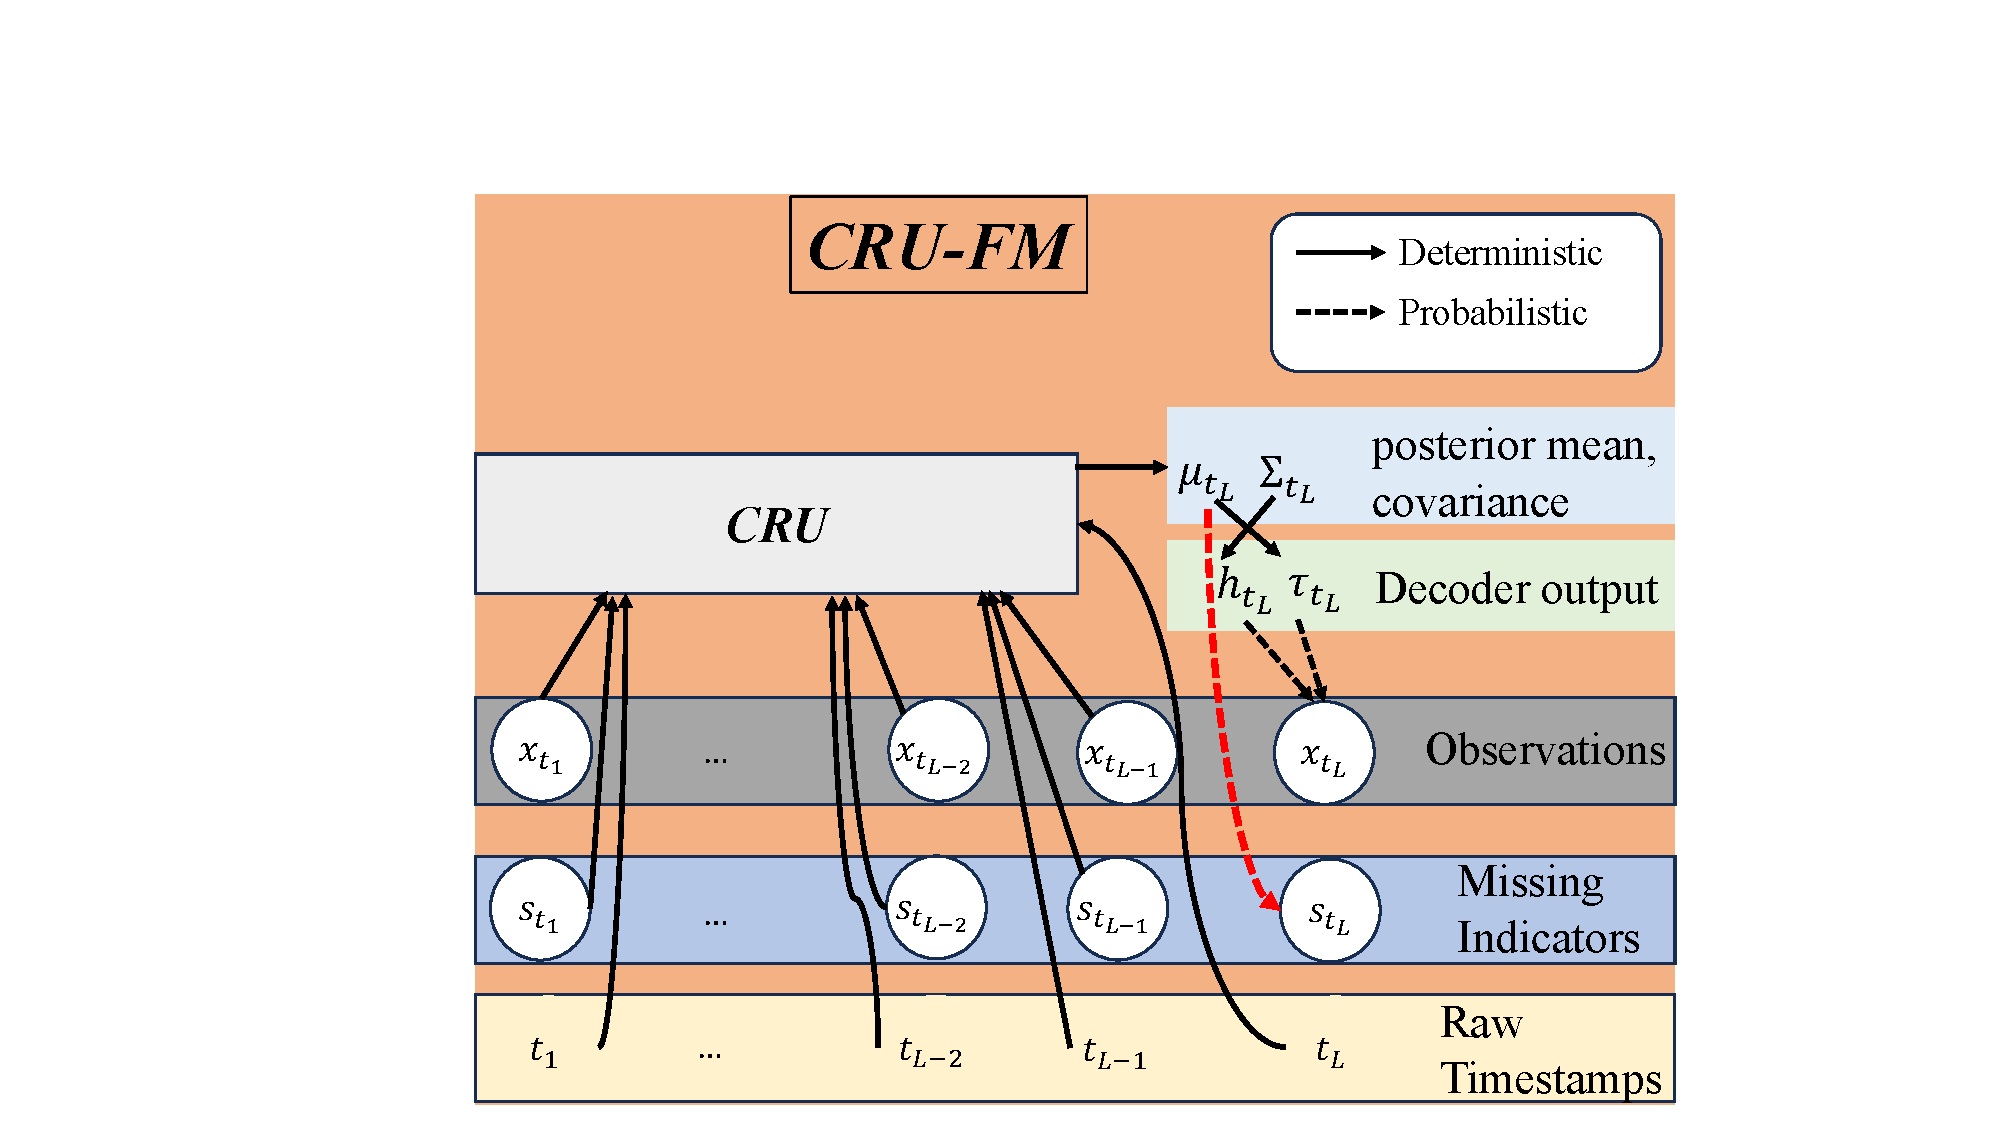
\includegraphics[width=0.9\textwidth]{content/chapters/irregular_time_series_data_driven_missingness/figures/cru_fm_diagram.pdf}
    \caption[Diagram of our proposed CRU-FM model]{Diagram of our CRU-FM model (Sec.~\ref{sec:CRU_gen_model}). We show the extrapolation generative process for data vector $x_{t_L}$ and binary seen/missing indicator $s_{t_L}$ at time $t_L$, conditioning on previous $x_{t_1:t_{L-1}}, s_{t_1:t_{L-1}}$.
    The red line highlights our contribution: a distribution on $s_{t_L}$ that is data-dependent and thus suitable for MAR settings. Dashed lines point to values that are sampled from a distribution, not deterministically computed from predecessors. 
    }%endcaption
    \label{fig:generative_model}
    % \vspace{-.7cm} %% HACK
\end{figure}
